\documentclass[11pt]{article}
\usepackage[paperwidth=13.333in,paperheight=7.5in,margin=0.25in]{geometry}
\pagestyle{empty}
\usepackage{tikz}
\usetikzlibrary{arrows.meta,positioning,fit,calc,shapes.geometric,backgrounds}
\usepackage{xcolor}
% The default palette is the white-background evidence-report style. The
% figure builder defines \DARKTHEME for slide-ready variants.
\ifdefined\DARKTHEME
\definecolor{ink}{HTML}{F3F7FA}
\definecolor{muted}{HTML}{B9C7D4}
\definecolor{grid}{HTML}{2B3B4B}
\definecolor{blue}{HTML}{62B8FF}
\definecolor{teal}{HTML}{55D6C2}
\definecolor{orange}{HTML}{FFBD5A}
\definecolor{red}{HTML}{FF7568}
\definecolor{purple}{HTML}{C3A6FF}
\definecolor{paleBlue}{HTML}{14283A}
\definecolor{paleOrange}{HTML}{3A2B14}
\definecolor{dataFill}{HTML}{241C3A}
\definecolor{modelFill}{HTML}{12352F}
\definecolor{specialistFill}{HTML}{3A2B14}
\definecolor{futureFill}{HTML}{1C2630}
\definecolor{pageBg}{HTML}{080D13}
\else
\definecolor{ink}{HTML}{102A43}
\definecolor{muted}{HTML}{52606D}
\definecolor{grid}{HTML}{D9E2EC}
\definecolor{blue}{HTML}{1976A8}
\definecolor{teal}{HTML}{16817A}
\definecolor{orange}{HTML}{D9822B}
\definecolor{red}{HTML}{C05640}
\definecolor{purple}{HTML}{6B5B95}
\definecolor{paleBlue}{HTML}{E8F1F5}
\definecolor{paleOrange}{HTML}{FFF1DF}
\definecolor{dataFill}{HTML}{F5F0FA}
\definecolor{modelFill}{HTML}{EAF6F4}
\definecolor{specialistFill}{HTML}{FFF1DF}
\definecolor{futureFill}{HTML}{F2F4F5}
\definecolor{pageBg}{HTML}{FFFFFF}
\fi
\pagecolor{pageBg}
\tikzset{
  base/.style={font=\sffamily, text=ink},
  title/.style={base, font=\sffamily\bfseries\fontsize{23}{27}\selectfont},
  subtitle/.style={base, font=\sffamily\fontsize{12}{15}\selectfont, text=muted},
  box/.style={base, rounded corners=3pt, draw=blue!65!black, fill=paleBlue, minimum height=0.78cm, minimum width=2.65cm, align=center, inner sep=7pt},
  data/.style={box, draw=purple!75!black, fill=dataFill},
  model/.style={box, draw=teal!75!black, fill=modelFill},
  specialist/.style={box, draw=orange!85!black, fill=specialistFill},
  future/.style={box, draw=muted, fill=futureFill, dashed},
  arrow/.style={-{Latex[length=3mm]}, line width=0.9pt, draw=muted},
  dashedarrow/.style={-{Latex[length=3mm]}, line width=0.8pt, draw=muted, dashed},
  note/.style={base, font=\sffamily\fontsize{18}{22}\selectfont, text=muted, align=left},
}

\begin{document}
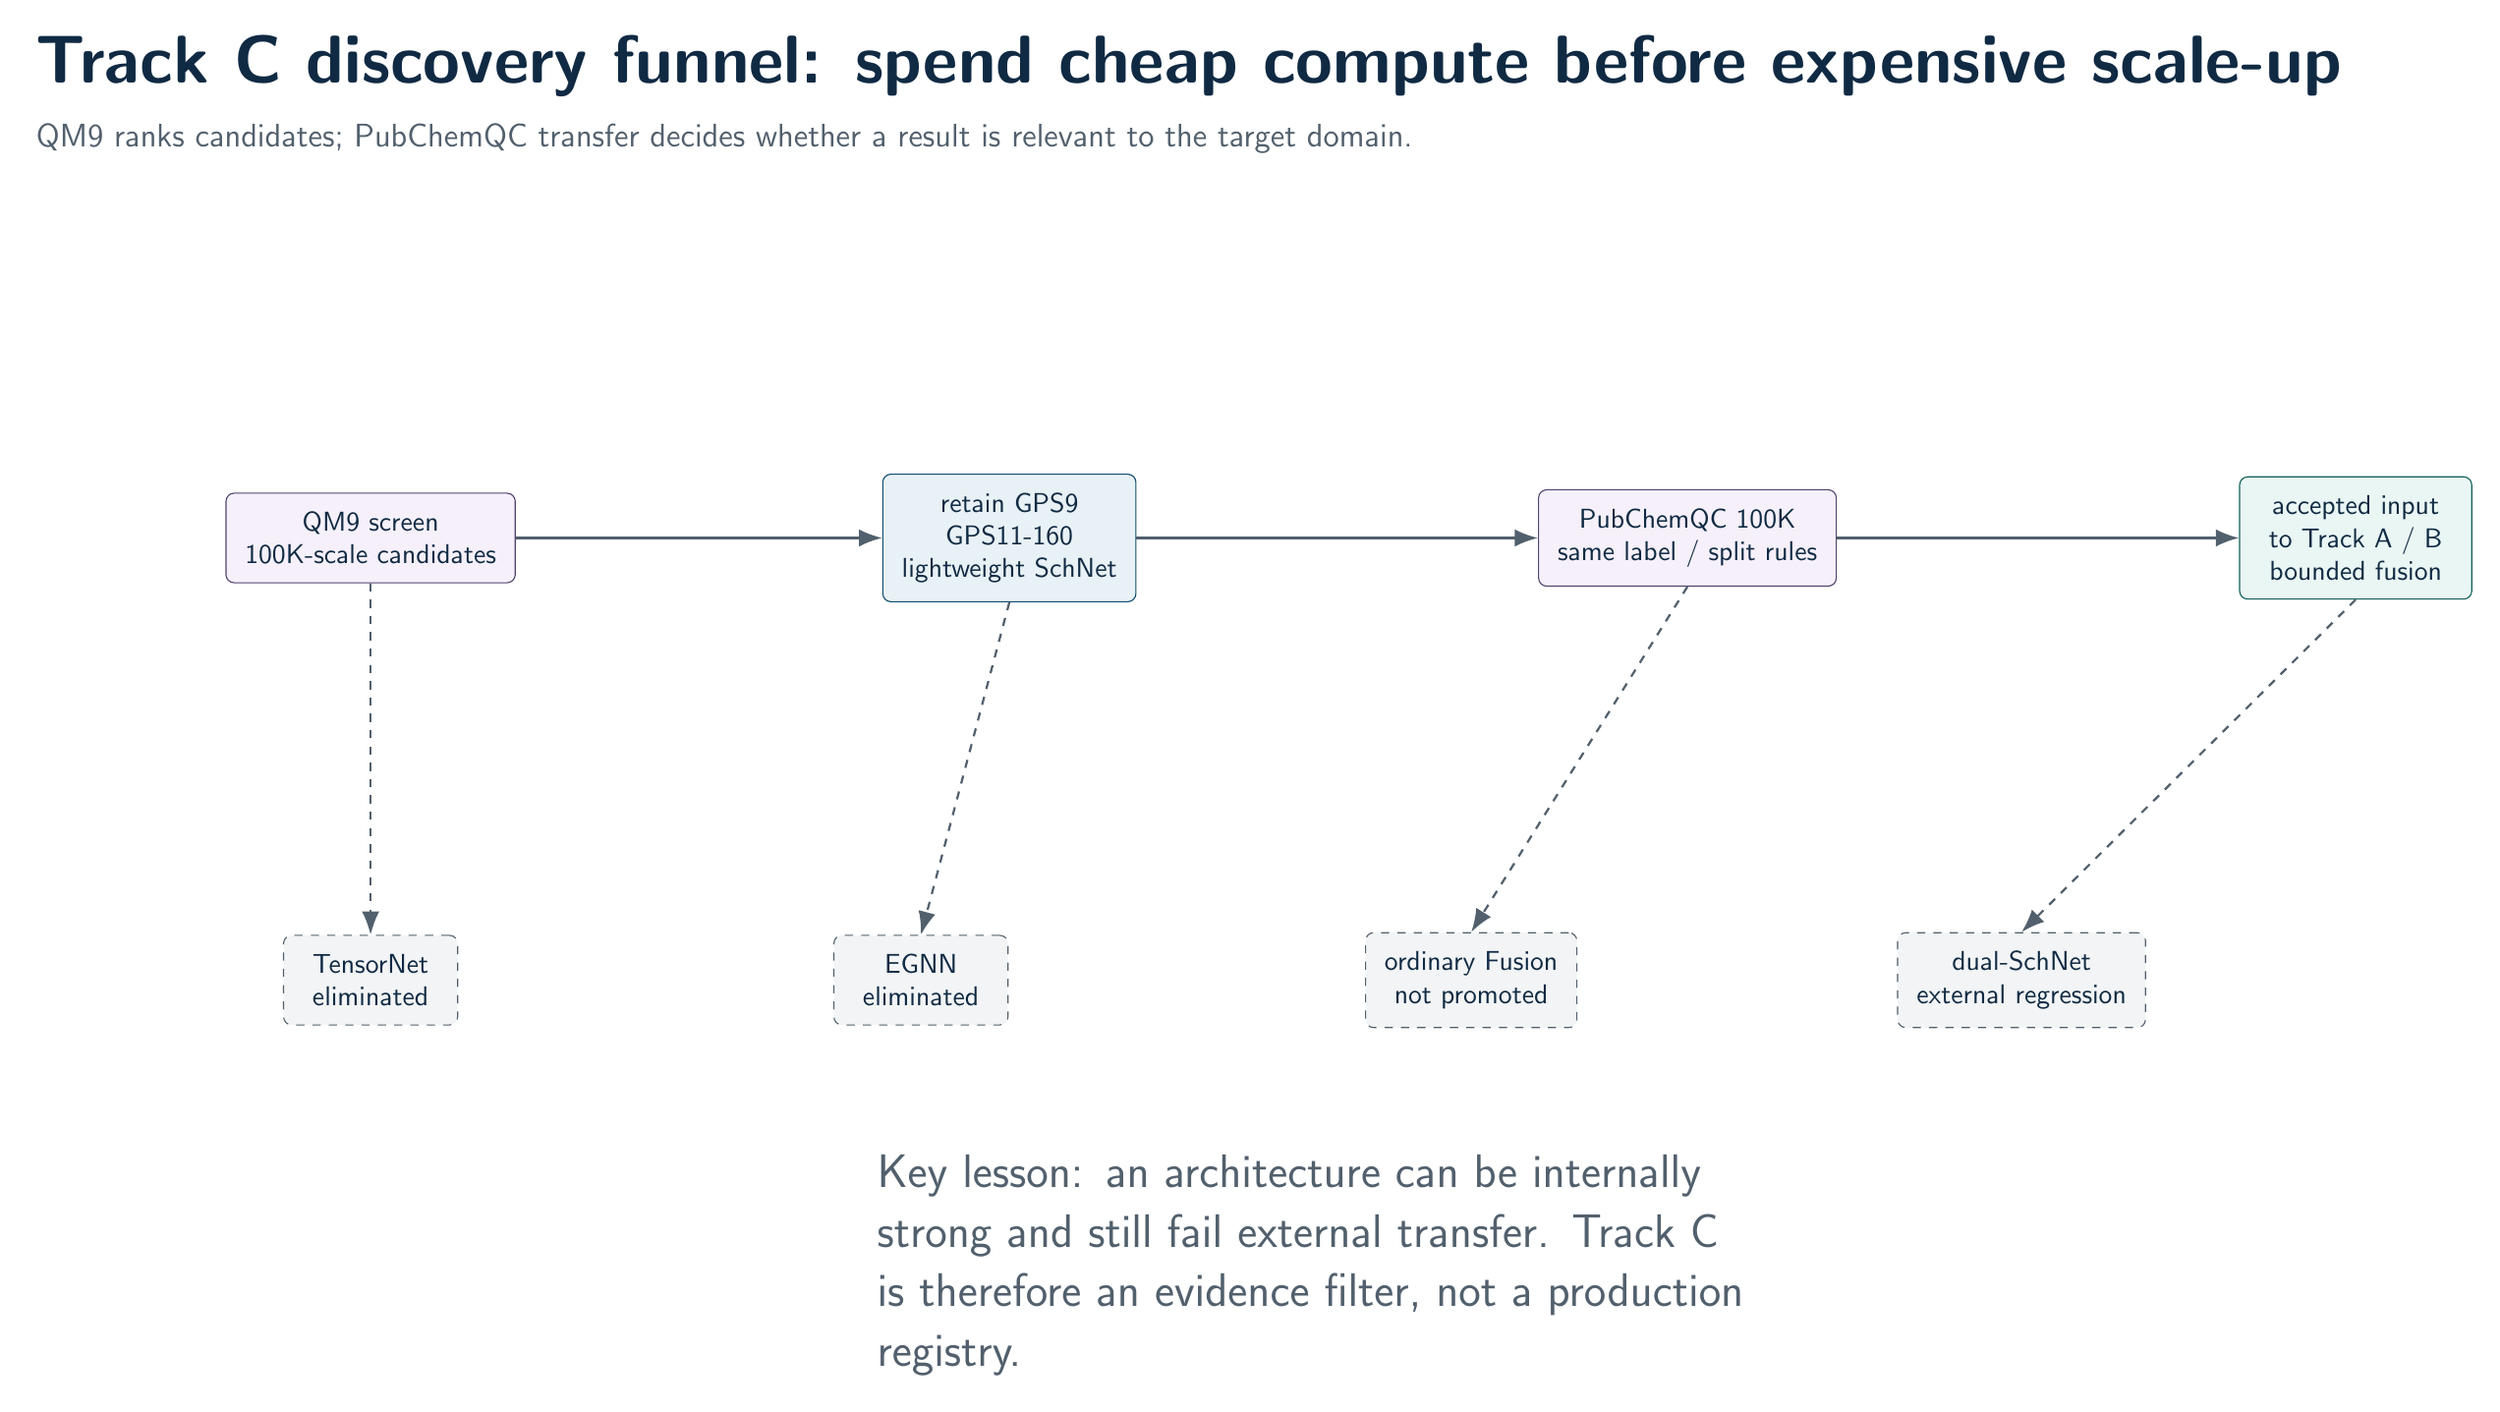
\begin{tikzpicture}[x=1in,y=1in]
  \node[title,anchor=west] at (0,6.85) {Track C discovery funnel: spend cheap compute before expensive scale-up};
  \node[subtitle,anchor=west] at (0,6.48) {QM9 ranks candidates; PubChemQC transfer decides whether a result is relevant to the target domain.};

  \node[data,minimum width=2.85cm,minimum height=1.0cm] (q) at (1.75,4.45) {QM9 screen\\100K-scale candidates};
  \node[box,minimum width=2.85cm,minimum height=1.0cm] (keep) at (5.0,4.45) {retain GPS9\\GPS11-160\\lightweight SchNet};
  \node[data,minimum width=3.0cm,minimum height=1.0cm] (t) at (8.45,4.45) {PubChemQC 100K\\same label / split rules};
  \node[model,minimum width=3.0cm,minimum height=1.0cm] (f) at (11.85,4.45) {accepted input\\to Track A / B\\bounded fusion};
  \draw[arrow] (q.east) -- (keep.west);
  \draw[arrow] (keep.east) -- (t.west);
  \draw[arrow] (t.east) -- (f.west);

  \node[future,minimum width=2.25cm,minimum height=0.8cm] (x1) at (1.75,2.2) {TensorNet\\eliminated};
  \node[future,minimum width=2.25cm,minimum height=0.8cm] (x2) at (4.55,2.2) {EGNN\\eliminated};
  \node[future,minimum width=2.25cm,minimum height=0.8cm] (x3) at (7.35,2.2) {ordinary Fusion\\not promoted};
  \node[future,minimum width=2.25cm,minimum height=0.8cm] (x4) at (10.15,2.2) {dual-SchNet\\external regression};
  \draw[dashedarrow] (q.south) -- (x1.north);
  \draw[dashedarrow] (keep.south) -- (x2.north);
  \draw[dashedarrow] (t.south) -- (x3.north);
  \draw[dashedarrow] (f.south) -- (x4.north);

  \node[note,text width=11.8cm] at (6.65,0.75) {Key lesson: an architecture can be internally strong and still fail external transfer. Track C is therefore an evidence filter, not a production registry.};
\end{tikzpicture}
\end{document}
